%%%%%%%%%%%%%%%%%%%%%%%%%%%%%%%%%%%%%%%%%%%%%%%%%%%%%%%%%%%%%%%%%%%%%%%%%
% This is the LaTeX template file for lecture notes for NWU CS496.
% Attribution: Modified from Berkeley EECS CS 294-8.
%%%%%%%%%%%%%%%%%%%%%%%%%%%%%%%%%%%%%%%%%%%%%%%%%%%%%%%%%%%%%%%%%%%%%%%%%

\documentclass{article}


%%%%%%%%%%%%%%%%%%%%%%%%%%%%%%%%%%%%%%%%%%%%%%%%%%%%%%%%%%%%%%%%%%%%%%%%%
%  Package declaration
%%%%%%%%%%%%%%%%%%%%%%%%%%%%%%%%%%%%%%%%%%%%%%%%%%%%%%%%%%%%%%%%%%%%%%%%%
\usepackage{color}
\usepackage{algorithm}
\usepackage{algorithmicx}
\usepackage{algpseudocode}
\usepackage{mathtools}
\usepackage{amsthm} % theorems, proofs, ...
\usepackage{amsmath,amsfonts,amssymb,graphicx}
\usepackage{subfigure}
\usepackage{tikz}
\usepackage{filecontents} % Inline bibliographies


%%%%%%%%%%%%%%%%%%%%%%%%%%%%%%%%%%%%%%%%%%%%%%%%%%%%%%%%%%%%%%%%%%%%%%%%%
%  Settings
%%%%%%%%%%%%%%%%%%%%%%%%%%%%%%%%%%%%%%%%%%%%%%%%%%%%%%%%%%%%%%%%%%%%%%%%%

\setlength{\oddsidemargin}{0.25 in}
\setlength{\evensidemargin}{-0.25 in}
\setlength{\topmargin}{-0.6 in}
\setlength{\textwidth}{6.5 in}
\setlength{\textheight}{8.5 in}
\setlength{\headsep}{0.75 in}
\setlength{\parindent}{0 in}
\setlength{\parskip}{0.1 in}


%%%%%%%%%%%%%%%%%%%%%%%%%%%%%%%%%%%%%%%%%%%%%%%%%%%%%%%%%%%%%%%%%%%%%%%%%
%  Commands
%%%%%%%%%%%%%%%%%%%%%%%%%%%%%%%%%%%%%%%%%%%%%%%%%%%%%%%%%%%%%%%%%%%%%%%%%
%
% The following commands are used to generate the header.
%
\newcounter{lecnum}
\newcommand{\lecture}[4]{
   \pagestyle{myheadings}
   \thispagestyle{plain}
   \newpage
   \setcounter{lecnum}{#1}
   \setcounter{page}{1}
   \noindent
   \begin{center}
   \framebox{
      \vbox{\vspace{2mm}
    \hbox to 6.28in { {\bf CS 496 Approximation Algorithms
                        \hfill Winter 2021} }
       \vspace{4mm}
       \hbox to 6.28in { {\Large \hfill Lecture #1: #2  \hfill} }
       \vspace{2mm}
       \hbox to 6.28in { {\it Lecturer: #3 \hfill Scribe: #4} }
      \vspace{2mm}}
   }
   \end{center}
   \markboth{Lecture #1: #2}{Lecture #1: #2}
   {\bf Disclaimer}: {\it These notes have not been subjected to the
   usual scrutiny reserved for formal publications.  They may be distributed
   outside this class only with the permission of the Instructor.}
   \vspace*{4mm}
}


% Use these for theorems, lemmas, proofs, etc.
\newtheorem{theorem}{Theorem}
\newtheorem{lemma}[theorem]{Lemma}
\newtheorem{remark}{Remark}
\newtheorem{fact}[theorem]{Fact}
\newtheorem{definition}[theorem]{Definition}
\newtheorem{corollary}[theorem]{Corollary}
\newtheorem{proposition}[theorem]{Proposition}
\newtheorem{claim}[theorem]{Claim}
\newtheorem{conjecture}[theorem]{Conjecture}
\newtheorem{observation}[theorem]{Observation}
\newtheorem{assumption}[theorem]{Assumption}
\newtheorem{example}[theorem]{Example}

% argmin and argmax
\DeclareMathOperator*{\argmax}{arg\,max}
\DeclareMathOperator*{\argmin}{arg\,min}

% Distances
\newcommand{\totalvardist}[2]{{\operatorname{d_{\rm TV}}\!\left({#1, #2}\right)}}
\newcommand{\hamming}[2]{{\operatorname{d}\!\left(#1, #2\right)}}
\newcommand{\editdist}[2]{{\operatorname{d}\!\left(#1, #2\right)}}
\newcommand{\dist}[2]{{\operatorname{dist}\!\left(#1, #2\right)}}

% Norms
\newcommand{\norm}[1]{\lVert#1{\rVert}}
\newcommand{\normone}[1]{{\norm{#1}}_1}
\newcommand{\normtwo}[1]{{\norm{#1}}_2}
\newcommand{\norminf}[1]{{\norm{#1}}_\infty}
\newcommand{\abs}[1]{\left\lvert #1 \right\rvert}

% Sets and indicators
\newcommand{\setOfSuchThat}[2]{ \left\{\; #1 \;\colon\; #2\; \right\} } 			% sets such as "{ elems | condition }"

% Probability
\newcommand{\proba}{\operatorname{\mathbb{P}}}
\newcommand{\probaOf}[1]{\Pr\!\left[\, #1\, \right]}
\newcommand{\probaCond}[2]{\Pr\!\left[\, #1 \;\middle\vert\; #2\, \right]}
\newcommand{\probaDistrOf}[2]{\Pr_{#1}\left[\, #2\, \right]}

% Expectation & variance
\newcommand{\expect}[1]{\mathbb{E}\!\left[#1\right]}
\newcommand{\expectCond}[2]{\mathbb{E}\!\left[\, #1 \;\middle\vert\; #2\, \right]}
\newcommand{\expectOn}[2]{\mathbb{E}_#1\!\left[#2\right]}
\newcommand{\expectCondOn}[3]{\mathbb{E}_#1\!\left[\, #2 \;\middle\vert\; #3\, \right]}
\newcommand{\shortexpect}{\mathbb{E}}
\newcommand{\var}{\operatorname{Var}}
\newcommand{\uniform}{\ensuremath{\mathcal{U}}}

% Complexity
\newcommand{\littleO}[1]{{o\!\left({#1}\right)}}
\newcommand{\bigO}[1]{{O\!\left({#1}\right)}}
\newcommand{\bigTheta}[1]{{\Theta\!\left({#1}\right)}}
\newcommand{\bigOmega}[1]{{\Omega\!\left({#1}\right)}}
\newcommand{\tildeO}[1]{\tilde{O}\!\left({#1}\right)}
\newcommand{\tildeTheta}[1]{\operatorname{\tilde{\Theta}}\!\left({#1}\right)}

%%%%%%%%%%%%%%%%%%%%%%%%%%%%%%%%%%%%%%%%%%%%%%%%%%%%%%%%%%%%%%%%%%%%%%%%%
%  Note header
%%%%%%%%%%%%%%%%%%%%%%%%%%%%%%%%%%%%%%%%%%%%%%%%%%%%%%%%%%%%%%%%%%%%%%%%%
\begin{document}
%\lecture{**LECTURE-NUMBER**}{**DATE**}{**LECTURER**}{**SCRIBE**}
\lecture{1}{January 1}{Konstantin Makarychev}{Muhan Li}

%%%%%%%%%%%%%%%%%%%%%%%%%%%%%%%%%%%%%%%%%%%%%%%%%%%%%%%%%%%%%%%%%%%%%%%%%
%  Note section

%  Important hint: be concise while describing, if something is too 
%  complex, use figures and graphs. However, while proving / using math
%  equations, include all necessary details, such as what inequality is
%  used, etc.
%%%%%%%%%%%%%%%%%%%%%%%%%%%%%%%%%%%%%%%%%%%%%%%%%%%%%%%%%%%%%%%%%%%%%%%%%

\section{An ordinary paragraph with inline equations}

The naive and obvious solution to All Pairs Shortest Path(APSP) problem is to
run a Single Source Shortest Path algorithm from each starting vertex
$v$.  If the graph has arbitrary edge weights, it takes the Bellman-Ford
algorithm $O(|E||V|^2)$ time to solve APSP.  But there
are better approaches.

\subsection{Multi-line equations}
In multi-line equations, use "\&" to vertically align your equations.

For equations without numbers. 
\begin{flalign*}
&\expectOn{y}{\sum_{x \in C} \min_{c \in \{c_1,...,c_t,y\}} \norm{x-c}^2} \\
&= \sum_{y \in C} \frac{cost_t(y)}{cost_t(C)} * \sum_{x \in C} \min\{cost_t(x), \norm{x-y}^2\} \\
&\text{(when you need to explain what happens here.)} \\
&\text{(eg: With hoeffding inequality, union bound, etc.)} \\
&= \sum_{x \in C, y \in C} \frac{cost_t(y)}{cost_t(C)} \min\{cost_t(x), \norm{x-y}^2\} \\
\end{flalign*}

For equations with numbers.
\begin{flalign}
2n + 1 &= \bigO{n} \\
f(x) &= \littleO{g(x)} \\
q(x) &= \bigTheta{p(x)} 
\end{flalign}



\section{Pesudo code}
We use the algorithmic package to write formal pesudo code.
\begin{algorithm}
	\caption{K-means (Floyd) algorithm}
	\label{K-means}
	\begin{algorithmic}[1] % The number tells where the line numbering should start
		\Procedure{K-means}{$D,k,T$} \Comment{$D = \{x_1,\ldots,x_n\}$, $k$ the cluster number, $T$ loop times.}
		\State Randomy select $k$ samples from $D$ as initial cluster centers $\{\mu_1,\ldots,\mu_k\}$
		\State $t \gets 0$.
		\Repeat					\Comment{Either do it with \textbackslash Repeat+ \textbackslash Until, or \textbackslash While + \textbackslash EndWhile}
		\State $t \gets t + 1$
		\State $C_i \gets \emptyset \ (1 \leq i \leq k)$
		\For{$j=1,\ldots,m$}
			\State $d_{ji} \gets \normtwo{x_j - u_i}$ \Comment{For each sample,, compute distance to every center.}
			\State $\lambda_j = \argmin_{i \in {1,\ldots,k}} d_{ji}$ \Comment{Determine cluster label of the sample.}
			\State $C_{\lambda_j} = C_{\lambda_j} \cup \{x_j\}$ \Comment{Assign sample to target cluster.}
		\EndFor
		\For{$i=1,2,...,k$}
			\State $\mu_i' \gets \frac{1}{|C_i|} \sum_{x \in C_i} x$ \Comment{Compute new centers.}
			\If{$\mu_i' \neq \mu_i$}	
				\State $\mu_i \gets \mu_i'$ \Comment{Update center value.}
			\Else
				\State Keep current center value.
			\EndIf
		\EndFor
		\State \Until{No more updates to centers or $t \geq T$.}
		\State \textbf{return $\mathcal{C} = \{C_1,\ldots,C_k\}$} \Comment{Return cluster partition}
		\EndProcedure
	\end{algorithmic}
\end{algorithm}

\section{Figures and tables}
By tradition, captions are put below figures and above tables. The label has to be placed either right after the caption or into the caption macro.

\begin{figure}[H]
	\centering
	\begin{tikzpicture}[] 
	\tikzstyle{level 1}=[sibling distance=60mm] 
	\tikzstyle{level 2}=[sibling distance=40mm] 
	\tikzstyle{level 3}=[sibling distance=20mm]
	\tikzstyle{level 4}=[sibling distance=20mm]
	\node [circle, draw] (x7)  {$x_7$} {
		child { node [circle, draw] (x5)  {$x_5$}
			child { node [circle, draw, fill=gray!15] (l1)  {$0$} }
			child { node [circle, draw, fill=gray!15] (l2)  {$1$} }
		}
		child { node [circle, draw] (x4)  {$x_4$}
			child { node [circle, draw] (x3)  {$x_3$}
				child { node [circle, draw, fill=gray!15] (l1)  {$1$} }
				child { node [circle, draw] (x1)  {$x_1$}
					child { node [circle, draw, fill=gray!15] (l1)  {$0$} }
					child { node [circle, draw, fill=gray!15] (l2)  {$1$} }
				}
			}
			child { node [circle, draw] (x5)  {$x_5$}
				child { node [circle, draw, fill=gray!15] (l1)  {$0$} }
				child { node [circle, draw] (x6)  {$x_6$}
					child { node [circle, draw, fill=gray!15] (l1)  {$1$} }
					child { node [circle, draw, fill=gray!15] (l2)  {$0$} }
				}
			}
		}
	};
	\end{tikzpicture}
	\caption{An example tikz picture.}
	\label{example-tikz}
\end{figure}

\begin{table}[H]
	\caption{An example table, with left align, center align, right align, and fixed size columns}.
	\label{example-table}
	\centering
	\begin{tabular}{ |l||r|c|p{3cm}|  }
		\hline
		\multicolumn{4}{|c|}{Country List} \\
		\hline
		Country Name     or Area Name& ISO ALPHA 2 Code &ISO ALPHA 3 Code&ISO numeric Code\\
		\hline
		Afghanistan   & AF    &AFG&   004\\
		Aland Islands&   AX  & ALA   &248\\
		Albania &AL & ALB&  008\\
		Algeria    &DZ & DZA&  012\\
		American Samoa&   AS  & ASM&016\\
		Andorra& AD  & AND   &020\\
		Angola& AO  & AGO&024\\
		\hline
	\end{tabular}
\end{table}

You can reference figure \ref{example-tikz} and Table \ref{example-table} like this.

\section{Citation}
Reference an article \cite{2021ox} and \cite{rizzo2021dynamical} like this.


%%%%%%%%%%%%%%%%%%%%%%%%%%%%%%%%%%%%%%%%%%%%%%%%%%%%%%%%%%%%%%%%%%%%%%%%%
%  Reference section
%%%%%%%%%%%%%%%%%%%%%%%%%%%%%%%%%%%%%%%%%%%%%%%%%%%%%%%%%%%%%%%%%%%%%%%%%
\begin{filecontents}{references1.bib}
@article{2021ox, 
	ISSN={1365-2966},
	url={http://dx.doi.org/10.1093/mnras/stab419},
	DOI={10.1093/mnras/stab419},
	journal={Monthly Notices of the Royal Astronomical Society},
	publisher={Oxford University Press (OUP)},
	year={2021}
}

@misc{rizzo2021dynamical,
	title={Dynamical properties of z $\sim 4.5$ dusty star-forming galaxies and their connection with local early type galaxies}, 
	author={Francesca Rizzo and Simona Vegetti and Filippo Fraternali and Hannah Stacey and Devon Powell},
	year={2021},
	eprint={2102.05671},
	archivePrefix={arXiv},
	primaryClass={astro-ph.GA}
}
	
\end{filecontents} 

%%%%%%%%%%%%%%%%%%%%%%%%%%%%%%%%%%%%%%%%%%%%%%%%%%%%%%%%%%%%%%%%%%%%%%%%%
%  Reference generation config
%  Do not change.
%%%%%%%%%%%%%%%%%%%%%%%%%%%%%%%%%%%%%%%%%%%%%%%%%%%%%%%%%%%%%%%%%%%%%%%%%
\nocite{*}
\bibliographystyle{alpha}
\bibliography{references1}

\end{document}




